\documentclass[a4paper]{article}
\usepackage[14pt]{extsizes} % для того чтобы задать нестандартный 14-ый размер шрифта
\usepackage[margin=0.7in]{geometry}
\usepackage{multirow}
\usepackage{graphicx}
\usepackage[utf8x]{inputenc} % указать кодировку русского текста
\usepackage[english, russian]{babel} % указать, что язык текста - русский
\usepackage{fancyhdr}
\pagestyle{fancy}
\usepackage{graphicx}
\usepackage{float}
\graphicspath{{pictures/}}
\DeclareGraphicsExtensions{.pdf,.png,.jpg}
\usepackage{tocloft}
\usepackage[T2A]{fontenc}
\usepackage{capt-of}
\usepackage[T2A]{fontenc}
\usepackage[utf8]{inputenc}
\usepackage[english,russian]{babel}
\usepackage{graphicx}
\usepackage{wrapfig}
\usepackage{mathtext} % русские буквы в фомулах
\usepackage{amsmath,amsfonts,amssymb,amsthm,mathtools} % AMS
\usepackage{icomma} % "Умная" запятая: $0,2$ —- число, $0, 2$ —- перечисление
\usepackage{capt-of}
\usepackage{appendix}
\usepackage{multirow}
\usepackage{hyperref}
\usepackage{multicol} % Несколько колонок
\usepackage{gensymb}


\graphicspath{ {images/} }
\usepackage{multicol}
\setlength{\columnsep}{2cm}


\renewcommand{\cftsecleader}{\cftdotfill{\cftdotsep}}
\begin{document} 
 \begin{titlepage}
\begin{center}
\hfill \break
Министерство науки и высшего образования Российской Федерации\\
ФЕДЕРАЛЬНОЕ ГОСУДАРСТВЕННОЕ АВТОНОМНОЕ ОБРАЗОВАТЕЛЬНОЕ\\ 
УЧРЕЖДЕНИЕ ВЫСШЕГО ОБРАЗОВАНИЯ\\ 
«МОСКОВСКИЙ ФИЗИКО-ТЕХНИЧЕСКИЙ ИНСТИТУТ\\ 
(НАЦИОНАЛЬНЫЙ ИССЛЕДОВАТЕЛЬСКИЙ УНИВЕРСИТЕТ)»\\
(МФТИ)\\
\hfill \break
\hfill \break
\hfill \break
\hfill \break
\hfill \break
\hfill \break
\hfill \break
\hfill \break
\hfill \break
\hfill \break
\hfill \break
КАФЕДРА ВАКУУМНОЙ ЭЛЕКТРОНИКИ\\
\hfill \break
ОТЧЕТ\\
ПО ЛАБОРАТОРНОЙ РАБОТЕ\\
\hfill \break
ДИОД ШОТТКИ\\
\end{center}
\hfill \break
\hfill \break
\hfill \break
\hfill \break
\hfill \break
\hfill \break
\hfill \break
\hfill \break
\begin{tabular}{ccc}
Работу выполнил студент  & \underline{\hspace{5cm}}&  \\\\
группы Б04-004& &   \\\\
 & &  \\\\
Работу принял, оценка & \underline{\hspace{5cm}} &  \\\\
\end{tabular}
\hfill \break
\hfill \break
\begin{center} Долгопрудный 2022 
\end{center}
\end{titlepage}

\section{Цель работы}
\begin{enumerate}
    \item Изучение применения диода в промышленности;
    \item Изучение физики процесса, наглядно убедиться в ее верности при помощи численного моделирования;
    \item Изготовление контакта Шоттки;
    \item Снятие характеристик изготовленного контакта, а также ранее изготовленного омического контакта.

\end{enumerate}

\section{Аннотация}

В работе изучается принцип работы диода Шоттки, который представляет собой выпрямитель напряжения.Также рассматриваются два вида контакта металла с полупроводником. Исследуемый диод Шоттки был сделан с помощью магнетронного напыления: изготовлен стек из материалов \textit{Al/Si/Au}. Для сравнение заранее был изготовлен омический контакт. В работе исследуются вольт-амперные характеристики изготовленных образцов и приводится сравнение полученных данных с характеристиками промышленных диодов. 

\section{Теоретические положения}
\subsection*{Практическое применение диода в промышленности}

Диоды являются одними из самых распространенных электронных компонентов. Они присутствуют практически во всех электронных приборах, которые мы ежедневно используем – от мобильного телефона до его зарядного устройства. Ниже рассмотрим основные типы электронных схем, в которых диоды нашли свое применение.

\textbf{1. Нелинейная обработка аналоговых сигналов.}
В связи с тем, что диоды относятся к элементам нелинейного типа, они применяются в детекторах, логарифматорах, экстрематорах, преобразователях частоты и в других устройствах, в которых предполагается нелинейная обработка аналоговых сигналов. В таких случаях диоды используют или как основные рабочие приборы – для обеспечения прохождения главного сигнала, или же в качестве косвенных элементов, например в цепях обратной связи. Указанные выше устройства значительно отличаются между собой и используются для разных целей, но применяемые диоды в каждом из них занимают очень важное место.

\textbf{2. Выпрямители.}
Устройства, которые используются для получения постоянного тока из переменного называются выпрямителями. В большинстве случаев они включают в себя три главных элемента – это силовой трансформатор, непосредственно выпрямитель (вентиль) и фильтр для сглаживания. Диоды применяют в качестве вентилей, так как по своим свойствам они отлично подходят для этих целей.

\textbf{3. Стабилизаторы.}
Устройства, которые служат для реализации стабильности напряжения на выходе источников питания, называются стабилизаторами. Они бывают разных видов, но каждый из них предполагает применение диодов. Эти элементы могут использоваться либо в цепях, отвечающих за опорные напряжения, либо в цепях, которые служат для коммутации накопительной индуктивности.

\textbf{4. Ограничители.}
Ограничители – это специальные устройства, используемые для того, чтобы ограничивать возможный диапазон колебания различных сигналов. В цепях такого типа широко применяются диоды, которые имеют прекрасные ограничительные свойства. В сложных устройствах могут использоваться и другие элементы, но большинство ограничителей базируются на самых обычных диодных узлах стандартного типа.

\textbf{5. Устройства коммутации.}
Диоды нашли применение и в устройствах коммутации, которые используются для того, чтобы переключать токи или напряжения. Диодные мосты дают возможность размыкать или замыкать цепь, которая служит для передачи сигнала. В работе применяется некоторое управляющее напряжение, под воздействием которого и происходит замыкание или размыкание. Иногда управляющим может быть сам входной сигнал, такое бывает в самых простых устройствах.

\textbf{6. Логические цепи.}
В логических цепях диоды применяются для того, чтобы обеспечить прохождение тока в нужном направлении (элементы «И», «ИЛИ»). Подобные цепи используются в схемах аналогового и аналогово-цифрового типа. Здесь перечислены только основные устройства, в которых применяются диоды, но существует и много других, менее распространенных.

\subsection*{Диод в цепи}

Однако из всех вышеприведенных способов применения диода в промышленности, главный из них - выпрямитель напряжения. Чтобы понять, как работает диод, рассмотрим простую цепь с диодом и без, затем изобразим зависимость напряжения от времени (рис.1)

\begin{center}
    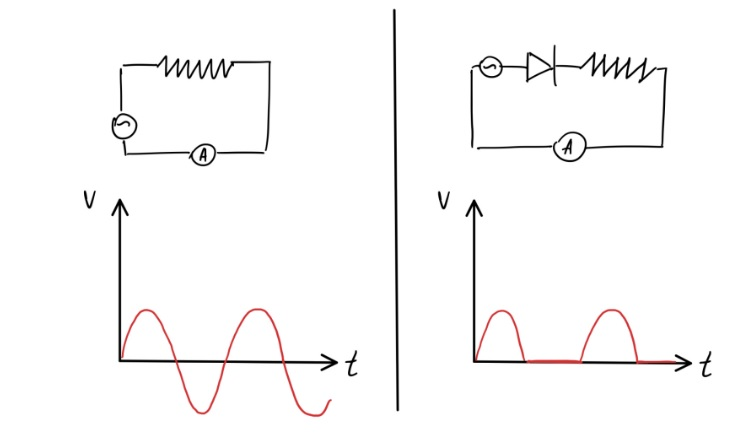
\includegraphics[scale = 0.7]{V(t).jpg}
    \captionof{figure}{Зависимость напряжения от времени в присутствии диода и в его отсутствие }
\end{center}

Т.к. рассматриваемый нами Диод представляет из себя контакт металла и полупроводника, то имеет смысл разобраться в природе полупроводников.

\subsection*{Энергетические диаграммы металла и полупроводника}
Для начала изобразим зонные диаграммы для металла и полупроводника (рис.2)
Здесь энергия, необходимая для выхода электрона в вакуум (далее работа выхода), находится как разность уровней вакуума и Ферми. Как видно из диаграммы, отличие полупроводника в наличии запрещенной зоны, в которой не может быть занятых состояний. Отсюда получаем, что уровень Ферми в полупроводнике находится между зонами валентности и проводимости.
Уровень Ферми также характеризуется заселенностью, равной 1/2, при любой температуре. Легко его можно найти их распределения Ферми-Дирака (1), которое дает информацию о вероятности нахождения электрона на уровне с энергией Е

\begin{center}
    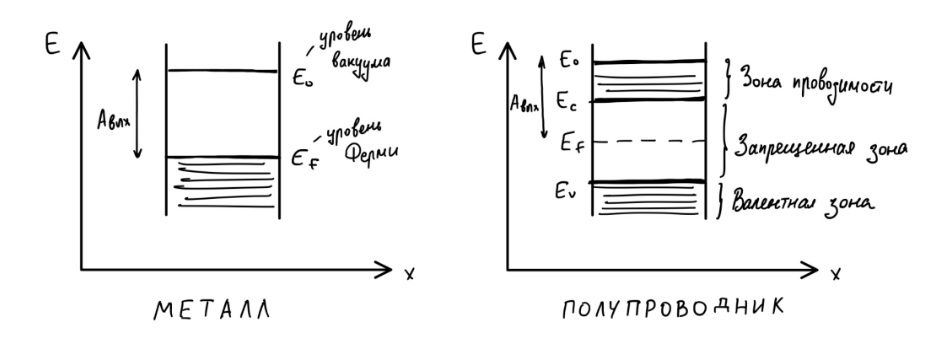
\includegraphics[scale = 0.7]{zonn_diag.jpg}
    \captionof{figure}{Зонная диаграммы металла и полупроводника }
\end{center}

\begin{equation}
	f(E) = \frac{1}{1+exp(\frac{E-E_{F}}{kT})} 
\end{equation}

Изобразим графики f(E) для металла и полупроводника (рис.3)

\begin{center}
    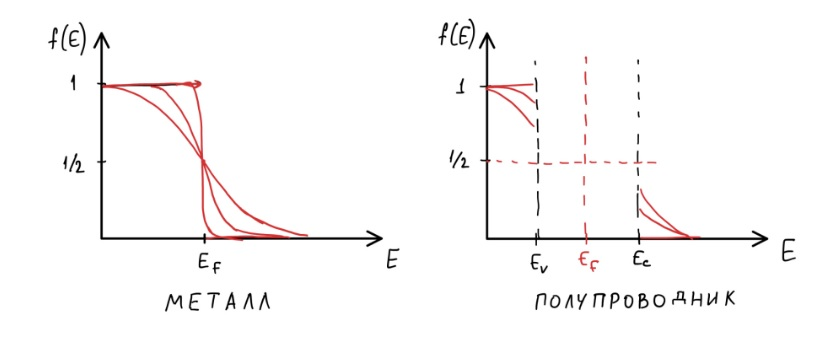
\includegraphics[scale = 0.7]{Ferm-Dir.jpg}
    \captionof{figure}{Графики распределения Ферми-Дирака для металла и полупроводника }
\end{center}
\subsection*{Полупроводник n-типа}
Полупроводник n-типа обладает донорной примесью (элементом с лишним электроном). Для примера рассмотрим фтор, который встраивается в структуру кремния (рис.4).
\begin{center}
    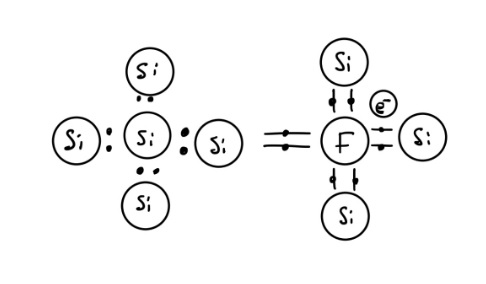
\includegraphics[scale = 0.7]{donor.jpg}
    \captionof{figure}{Донорный фтор в структуре кремния }
\end{center}
Так фтор дает в запрещенной зоне дополнительный уровень, находящийся блозко к зоне проводимости. Тогда необходимо приложить небольшую температуру (обычно комнатной достаточно), чтобы электрон с донорного уровня перешел в зону проводимости. Понятно, что тогда распределение Ферми-Дирака примет немного другой вид (рис.5).

\newpage
\begin{center}
    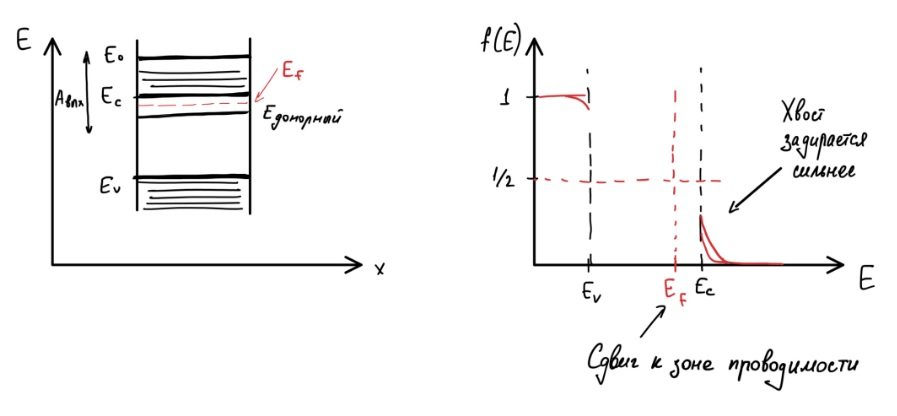
\includegraphics[scale = 0.7]{n-type.jpg}
    \captionof{figure}{Характеристики проводника n-типа }
\end{center}

\subsection*{Полупроводник p-типа}
Аналогичный принцип работы у акцепторных примесей, который не отдают электрон, а принимают. Тогда в запрещенной зоне возникает дополнительный акцепторный уровень, который находится ближе к зоне валентности. Вследствие этого уровень Ферми смещается ближе к зоне валентности и находится между данной зоной и акцепторным уровнем (рис.6).
\begin{center}
    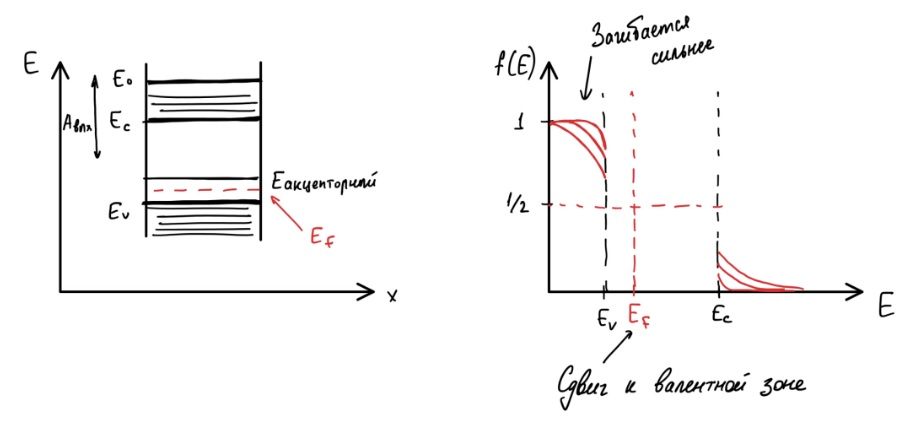
\includegraphics[scale = 0.7]{p-type.jpg}
    \captionof{figure}{Характеристики проводника p-типа }
\end{center}
\subsection*{Диод Шоттки}
Рассмотрим контакт полупроводника n-типа и металла. Пусть работа выхода полупроводника меньше, чем у металла. Тогда на границе полупроводник-металл образуется скачок напряжения (барьер):
\begin{equation}
	U_{barrier} = \frac{A_{m}-A{s}}{q} .
\end{equation}

Как известно, при контакте двух материалов, их уровни Ферми должны сравняться. При этом остальные уровни опускаются, вследствие чего и образуется барьер (рис.7)
\begin{center}
    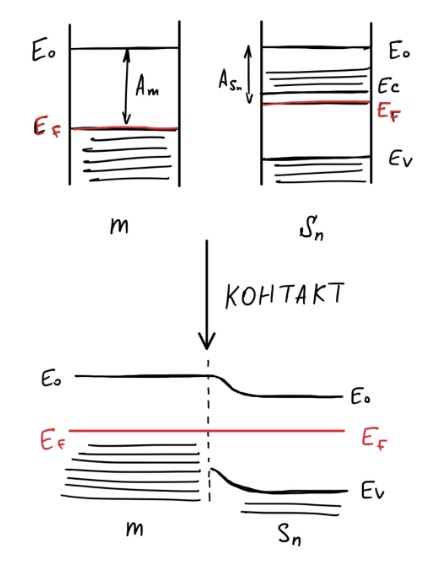
\includegraphics[scale = 0.7]{barrier.jpg}
    \captionof{figure}{Образование барьера при контакте металл-полупроводник n-типа}
\end{center}
Таким образом мы получаем не только выпрямление напряжения, но и основную отличительную способность диода: пропускать ток только в одну сторону. Это возникает, потому что при определенной полярности обеднение электронами у полупроводника на границе увеличивается, барьер растет, вследствие чего тока нет.
\subsection*{Омический контакт}
Омический контакт отличается тем, что работы выхода полупроводника и металла равны. Рассмотрим полупроводник n-типа и металл. Нарисуем для них зонные диаграммы (рис.8).
\begin{center}
    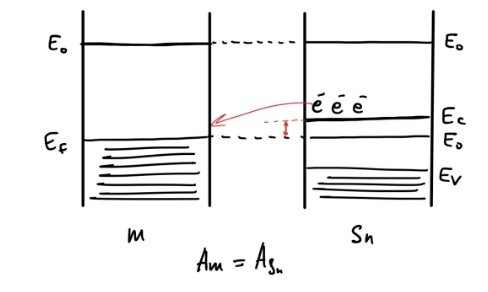
\includegraphics[scale = 0.7]{om_contact.jpg}
    \captionof{figure}{Зонная диаграмма при омическом контакте}
\end{center}
Отсюда видно, что при переходе из полупроводника в металл проблем нет, а в обратную сторону - электроны преодолевают барьер.

\section{Ход работы}
\subsection{Изготовление диода}

Диод представляет из себя кремниевую пластину, легированную бором (pSi) с концентрацией порядка $10^{15}-10^{16}$ см$^{(-3)}$, с одной стороны которого напылено золото (Au), с другой - алюминий (Al)
Изготовление производилось на установке ВНУ BOC Edwards AUTO 500 (далее AUTO 500) и ЭЛН Plassys MEB 550S (далее MEB 550S) (рис. 9 и 10) [2], [3] \\
\begin{center}
    \includegraphics[scale = 0.2]{Auto 500.jpg}
    \captionof{figure}{ВНУ BOC Edwards AUTO 500}
\end{center}
\begin{center}
    \includegraphics[scale = 0.1]{MEB550S Plassys.jpg}
    \captionof{figure}{ЭЛН Plassys MEB 550S}
\end{center}

Установка AUTO 500 оснащена высокочастотным магнетроном, магнетроном постоянного тока и системой электроннолучевого напыления. Для изготовления использовался высокочастотный магнетрон, однако данная установка имеет один существенный для наших целей недостаток: в трубку подачи аргона (аргон нужен для увеличения скорости напыления) подтекает воздух, из-за чего вместо алюминия напыляется его оксид, что влияет на качество диода, что будет отражено на графиках далее. \\

Откачивание до рабочего давления ($5*10^{-5}$ Торр при предельном $1*10^{-6}$ Торр) заняло порядка 90 минут, после чего было произведено напыление алюминия (золото было напылено заранее на установке MEB 550S) с подачей аргона.

Также был изготовлен омический контакт Au-pSi-Au

\newpage{}

\subsection{Снятие вольт-амперной характеристики (ВАХ)}

Снятие ВАХ производится на зондовой станции Cascade Microtech Summit 11000M.[4] \\
Полученные результаты:
\begin{center}
    \includegraphics[scale = 1.2]{1N5822.png}
    \captionof{figure}{ВАХ промышленного диода 1N5822}
\end{center}

\begin{center}
    \includegraphics[scale = 0.7]{bruh2.png}
    \captionof{figure}{ВАХ изготовленного диода}
\end{center}

%Здесь надо что-то умное спиздануть по поводу графиков%
Предварительные выводы:
\begin{enumerate}
    \item У изготовленного диода Шоттки при обратном напряжении около 1 В пробоя не происходит, однако на рис. 12 видно, что график не полностью ложится на ось абсцисс, и при обратном U = 1 B начинает уходить вниз. Был получен неидеальный диод. Открывающее напряжение - U ≈ - 0,1 В, коэффициент наклона аппроксимирующей прямой ≈ 47,9 мкА/В;                              
    \item Промышленный диод Шоттки: при обратном напряжении ∼ 8 В
    пробоя не происходит; открывающее напряжение ∼ 0,2 В; коэффициент
    наклона аппроксимирующей прямой ≈ 2,65 А/В;
    \item Исходя из полученных результатов можно сделать вывод, что промышленный диод Шоттки по всем характеристикам превосходит изготовленный (напряжения пробоя ≈ в 8 больше, коэффициент наклона прямой больше на 4 порядка, открывающее напряжение больше нуля).
\end{enumerate}
\section{Вывод}

В данной работе мы изучили принципы взаимодействия проводников и полупроводников с помощью зонных диаграмм, принципы работы диодов, а также экспериментально (посредством изготовления диода Шоттки, основанного на контакте полупроводника n-типа и металла) проверили данные законы.

\section{Литература}
1. \\
2. https://mipt.ru/science/labs/sec\_nanotechnology/oborudovanie/boc-edwards-auto-500/ \\
3. https://mipt.ru/about/departments/ckpn/eln-plassys-meb-550s/ \\
4. https://mipt.ru/about/departments/ckpn/zondovaya-stantsiya-summit-11000m/ \\

\end{document}
